\chapter{Validácia metodiky na simulovaných údajoch}
\label{chapter:vysledky}

\begin{quote}
\textbf{Upozornenie.} Všetky číselné hodnoty v tejto kapitole pochádzajú zo \emph{simulovaných} údajov. Nejde o výsledky výskumu a nemožno ich tak interpretovať. Účelom kapitoly je overiť, že analytický plán funguje: že dokáže z dát obnoviť parametre, z ktorých boli vygenerované, že rozlíši prítomnosť účinku od jeho neprítomnosti, a že pri plánovanej veľkosti vzorky poskytne rozhodnuteľnú odpoveď. Skutočné výsledky budú predmetom druhej časti práce.
\end{quote}

\section{Prečo simulovať pred zberom údajov}

Analytický plán je v empirickej práci rovnako náchylný na chyby ako softvér, a rovnako ako softvér sa dá otestovať. Napísaný, ale nespustený plán je nepreskúšaný kód. Postup použitý v tejto práci má tri kroky:

\begin{enumerate}[nosep]
    \item \textbf{Model generujúci dáta.} Zapíšeme hypotézy H1--H8 ako explicitný pravdepodobnostný model so známymi hodnotami parametrov, ukotvenými v efektoch z literatúry (časť~\ref{sec:dgp-kotvy}).
    \item \textbf{Spustenie plánu.} Na dátach z tohto modelu spustíme celý štatistický plán tak, ako bude spustený na reálnych dátach~--- bez akejkoľvek úpravy.
    \item \textbf{Porovnanie s pravdou.} Overíme, či odhady zodpovedajú vloženým hodnotám a či rozhodnutia (zamietnuť, nezamietnuť, vyhlásiť ekvivalenciu) vychádzajú správne.
\end{enumerate}

Tento postup už priniesol šesť konkrétnych opráv, ktoré by sa inak odhalili až po zbere dát, teda v okamihu, keď je náprava nemožná. Dve z nich sa týkali samotnej formulácie hypotéz a jedna by spôsobila, že primárny ukazovateľ by nemeral to, čo tvrdí. Sú uvedené v časti~\ref{sec:co-odhalila-simulacia}.

\section{Ukotvenie generujúceho modelu}
\label{sec:dgp-kotvy}

Parametre generujúceho modelu nie sú zvolené tak, aby vyšli pekné výsledky. Sú odvodené z publikovaných účinkov (tabuľka~\ref{tab:kotvy}). Tam, kde literatúra uvádza relatívne zmeny, sme ich konzervatívne prepočítali na štandardizované rozdiely a kde bolo možné, hodnotu sme zmenšili.

\begin{table}[H]
\centering
\caption{Ukotvenie parametrov generujúceho modelu v literatúre}
\label{tab:kotvy}
\small
\begin{tabularx}{\textwidth}{@{}l l X@{}}
\toprule
\textbf{Parameter} & \textbf{Hodnota} & \textbf{Zdroj a odôvodnenie} \\
\midrule
výkon počas hodiny $G$ vs. $K$ & $+0{,}22$ & Bastani a kol.~\cite{bastani2025harm}: $+48$\,\% relatívne \\
výkon počas hodiny $A$ vs. $K$ & $+0{,}33$ & tamže: $+127$\,\%, tlmené stropovým efektom \\
okamžitý test $A$ vs. $K$ & $+0{,}46\,\theta$ & Kestin a kol.~\cite{kestin2025aitutoring}, konzervatívne znížené \\
odložený test $G$ vs. $K$ & $-0{,}08\,\theta$ & Bastani a kol.: $-17$\,\% na následnom teste \\
odložený test $A$ vs. $K$ & $+0{,}34\,\theta$ & tamže: GPT Tutor nepoškodzuje, mierne pomáha \\
kalibračné skreslenie $G$ & $+0{,}23$ & Deslauriers a kol.~\cite{deslauriers2019feeling}, plynulosť \\
PEQI $\to$ odložený test & $+0{,}22$ & ICAP~\cite{chi2014icap}; sila zvolená konzervatívne \\
vnútrotriedna korelácia & $0{,}12$ & Hedges a Hedberg~\cite{hedges2007icc} \\
korelácia opakovaných meraní & $0{,}55$ & typická hodnota pre školské testy \\
úbytok do odloženého testu & $12$\,\% & skúsenosť z porovnateľných školských štúdií \\
\bottomrule
\end{tabularx}
\end{table}

Simulácia prebieha na úrovni jednotlivých položiek: latentná schopnosť sa prevádza na správne či nesprávne odpovede Raschovým modelom, a položková sebadôvera sa generuje z modelu využitia vodidiel~\cite{koriat1997monitoring} ako funkcia subjektívnej plynulosti. Vďaka tomu analýza pracuje s rovnakým typom vstupu, aký dostane v skutočnosti, vrátane chyby merania.

\section{Psychometrické vlastnosti testov}

Prvá vec, ktorú plán overuje, je, či sú testy dosť dlhé a dosť dobre rozložené. Tabuľka~\ref{tab:psychometria} ukazuje výsledok pre plánovanú vzorku 18~tried.

\begin{table}[H]
\centering
\caption{Psychometrické vlastnosti testových foriem ($J=18$, simulované údaje)}
\label{tab:psychometria}
\footnotesize
\begin{tabular}{@{}lccccc@{}}
\toprule
\textbf{Test} & \textbf{Položiek} & \textbf{Úspešnosť} & \textbf{Obtiažnosť} & \textbf{Spoľahl.} & \textbf{Separácia} \\
\midrule
IPT (okamžitý) & 16 & \psyIptP & $[\psyIptBlo;\ \psyIptBhi]$ & \psyIptRel & \psyIptSep \\
DRT (odložený) & 12 & \psyDrtP & $[\psyDrtBlo;\ \psyDrtBhi]$ & \psyDrtRel & \psyDrtSep \\
TT (transfer)  &  6 & \psyTtP & $[\psyTtBlo;\ \psyTtBhi]$ & --- & --- \\
\bottomrule
\end{tabular}
\vspace{2pt}
\footnotesize IPT a DRT sú kalibrované súbežne cez šesť kotviacich položiek, teda na jednej škále (22 položiek spolu). Koeficient $\alpha$ pre IPT je $\psyIptAlpha$.
\end{table}

Priemerná úspešnosť sa vo všetkých troch formách drží v cieľovom pásme ($0{,}30$ až $0{,}80$), takže nehrozí stropový ani podlahový efekt. Obnovenie parametrov Raschovho modelu je veľmi dobré pre obtiažnosti položiek ($r=\psyRecItem$) a primerané pre osobné miery ($r=\psyRecTheta$); zvyšný rozdiel je chyba merania, ktorá bude prítomná aj v skutočnosti.

Spoľahlivosť odloženého testu $\psyDrtRel$ je prijateľná. Stojí za zmienku, že súbežná kalibrácia ju oproti samostatnej zvýšila o niekoľko stotín: kotviace položky prinášajú informáciu z okamžitej príležitosti, takže odložený test sa meria presnejšie, než by mu jeho vlastných dvanásť položiek dovolilo. Útlm odhadov chybou merania tým neprestáva existovať~--- účinky na odloženom teste zostávajú podhodnotené približne o pätinu~--- ale je menší, než sa pri pôvodnom návrhu javilo.

\paragraph{Zhoda položiek s modelom.} Žiadna zo šestnástich položiek okamžitého testu nevypadla z pásma $0{,}7$ až $1{,}3$: infit sa pohybuje medzi $\psyInfitLo$ a $\psyInfitHi$, outfit medzi $\psyOutfitLo$ a $\psyOutfitHi$. Vylučovacie pravidlo z časti~\ref{sec:sap} teda na týchto dátach nič nevylúčilo, čo je očakávané, keďže dáta boli vygenerované Raschovým modelom. Jeho zmysel je opačný: na reálnych dátach dá vedieť, ak niektorá položka meria niečo iné než ostatné.

\paragraph{Funkčná odlišnosť položiek.} Najväčší posun obtiažnosti medzi podmienkami $A$ a $G$ je $\psyDifMax$ logitu, teda všetkých \psyDifNegligible{} položiek spadá do pásma zanedbateľnej odlišnosti. Rozdiel medzi podmienkami na týchto dátach teda nie je artefaktom nástroja.

\paragraph{Overenie ekvivalencie foriem.}
\label{sec:ekvivalencia-overenie}
Toto je kontrola, na ktorej stojí primárny ukazovateľ. Skutočný pokles latentnej schopnosti medzi okamžitou a odloženou príležitosťou bol vo generujúcom modeli $\psyDropTrue$ logitu. Súbežná kalibrácia ho odhadla na $\psyDropEst$, teda s chybou $\psyDropErr$. Veľkosť zabudnutia je preto merateľná, nie iba predpokladaná. Bez kotviacich položiek by táto hodnota bola artefaktom toho, ktorý test vyšiel ťažší, a tvrdenie o retencii by nebolo overiteľné vôbec.

\section{Obnovenie vložených účinkov}

\begin{table}[H]
\centering
\caption{Porovnanie vložených a odhadnutých účinkov (v jednotkách $d$)}
\label{tab:obnovenie}
\small
\begin{tabular}{@{}llcc@{}}
\toprule
\textbf{Ukazovateľ} & \textbf{Kontrast} & \textbf{Vložené} & \textbf{Odhadnuté} \\
\midrule
okamžitý test   & $A-K$ & $\recImmAKTarget$ & $\recImmAKEst$ \\
odložený test   & $A-K$ & $\recDelAKTarget$ & $\recDelAKEst$ \\
odložený test   & $G-K$ & $\recDelGKTarget$ & $\recDelGKEst$ \\
PEQI $\to$ odložený test & dráha $b$ & $\recPeqiTarget$ & $\recPeqiEst$ \\
kalibračné skreslenie & $G-K$ & $\recJolGtarget$ & $\recJolGest$ \\
kalibračné skreslenie & $A-K$ & $\recJolAtarget$ & $\recJolAest$ \\
\bottomrule
\end{tabular}
\end{table}

Plán obnovuje vložené hodnoty správne čo do smeru, poradia aj približnej veľkosti. Systematické podhodnotenie učebných účinkov (napríklad $\recImmAKEst$ oproti vloženým $\recImmAKTarget$) je očakávané a ide o útlm spôsobený chybou merania, nie o chybu v pláne. Z toho vyplýva dôležitý dôsledok pre plánovanie: aby bolo možné zachytiť účinok skutočnej veľkosti $d=0{,}30$, musí byť plán dimenzovaný na pozorovaný účinok približne $d=0{,}25$.

\section{Očakávaný obrazec výsledkov}

Obrázok~\ref{fig:ocakavane} zobrazuje, ako by vyzerali výsledky, ak platí zjednocujúca hypotéza z časti~\ref{sec:syntezahypotezy}. Práve tento obrazec je tým, čo výskum testuje~--- a čo môže vyjsť aj inak.

\begin{figure}[H]
    \centering
    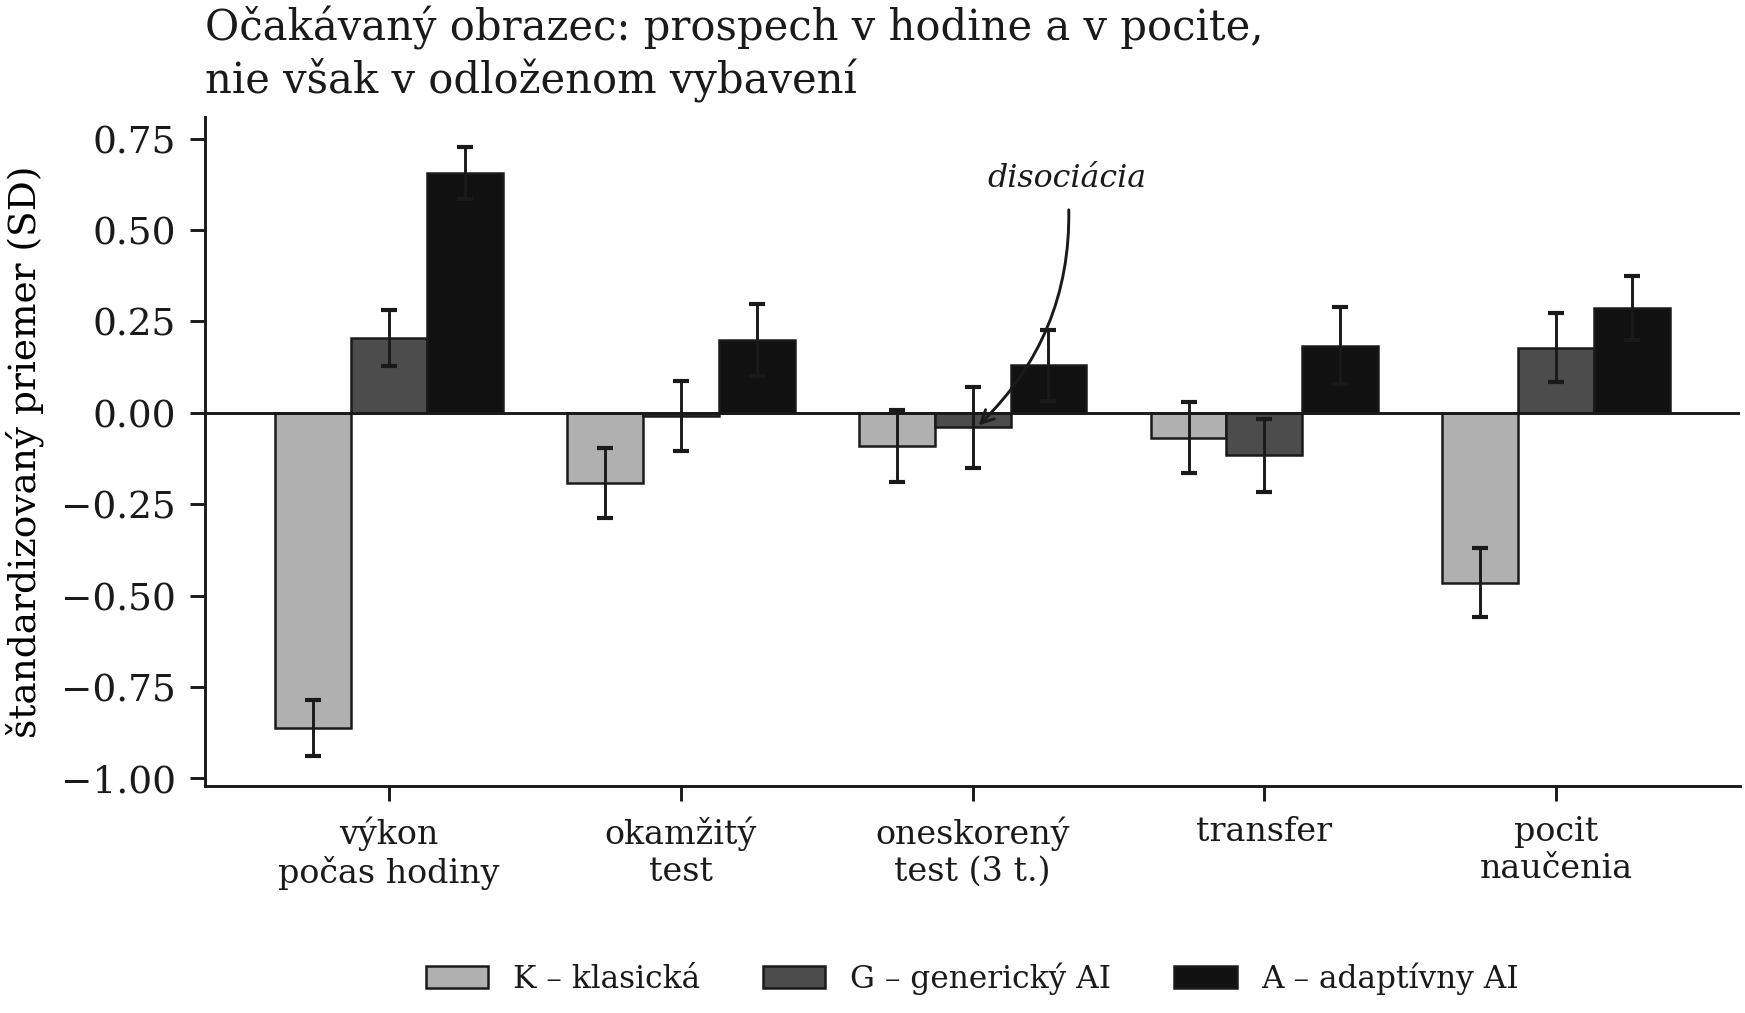
\includegraphics[width=\textwidth]{assets/images/fig_expected.png}
    \caption{Očakávaný obrazec. Obe podmienky s nástrojom výrazne prekonávajú klasickú výučbu počas hodiny aj v subjektívnom pocite naučenia; na odloženom teste sa však generický nástroj prepadá na úroveň klasickej výučby alebo pod ňu, zatiaľ čo adaptívny si výhodu udrží.}
    \label{fig:ocakavane}
\end{figure}

\begin{table}[H]
\centering
\caption{Kontrasty na simulovaných údajoch ($J=\numNclasses$, $N=\numNstudents$ zapísaných, $n=\numNcomplete$ s kompletnými dátami)}
\label{tab:kontrasty}
\small
\begin{tabular}{@{}llrrrr@{}}
\toprule
\textbf{Ukazovateľ} & \textbf{Kontrast} & \textbf{Odhad} & \textbf{SE} & \textbf{$d$} & \textbf{95\,\% IS} \\
\midrule
výkon počas hodiny & $G-K$ & $\conPracGK$ & \conPracGKSe & $\conPracGKD$ & $[\conPracGKLo;\ \conPracGKHi]$ \\
výkon počas hodiny & $A-K$ & $\conPracAK$ & \conPracAKSe & $\conPracAKD$ & $[\conPracAKLo;\ \conPracAKHi]$ \\
\midrule
okamžitý test & $A-K$ & $\conImmAK$ & \conImmAKSe & $\conImmAKD$ & $[\conImmAKLo;\ \conImmAKHi]$ \\
okamžitý test & $G-K$ & $\conImmGK$ & \conImmGKSe & $\conImmGKD$ & $[\conImmGKLo;\ \conImmGKHi]$ \\
okamžitý test & $A-G$ & $\conImmAG$ & \conImmAGSe & $\conImmAGD$ & $[\conImmAGLo;\ \conImmAGHi]$ \\
\midrule
\textbf{odložený test} & $\mathbf{A-K}$ & $\mathbf{\conDelAK}$ & \conDelAKSe & $\conDelAKD$ & $[\conDelAKLo;\ \conDelAKHi]$ \\
\textbf{odložený test} & $\mathbf{G-K}$ & $\mathbf{\conDelGK}$ & \conDelGKSe & $\conDelGKD$ & $[\conDelGKLo;\ \conDelGKHi]$ \\
\textbf{odložený test} & $\mathbf{A-G}$ & $\mathbf{\conDelAG}$ & \conDelAGSe & $\conDelAGD$ & $[\conDelAGLo;\ \conDelAGHi]$ \\
\midrule
transfer & $A-K$ & $\conTtAK$ & \conTtAKSe & $\conTtAKD$ & $[\conTtAKLo;\ \conTtAKHi]$ \\
transfer & $G-K$ & $\conTtGK$ & \conTtGKSe & $\conTtGKD$ & $[\conTtGKLo;\ \conTtGKHi]$ \\
transfer & $A-G$ & $\conTtAG$ & \conTtAGSe & $\conTtAGD$ & $[\conTtAGLo;\ \conTtAGHi]$ \\
\midrule
pocit naučenia & $G-K$ & $\conFolGK$ & \conFolGKSe & $\conFolGKD$ & $[\conFolGKLo;\ \conFolGKHi]$ \\
pocit naučenia & $A-K$ & $\conFolAK$ & \conFolAKSe & $\conFolAKD$ & $[\conFolAKLo;\ \conFolAKHi]$ \\
spokojnosť & $G-K$ & $\conSatGK$ & \conSatGKSe & $\conSatGKD$ & $[\conSatGKLo;\ \conSatGKHi]$ \\
\bottomrule
\end{tabular}
\vspace{2pt}
\footnotesize Tri riadky konfirmačnej rodiny sú vyznačené tučne. $N$ je počet žiakov v jednom náhodnom výbere generujúceho modelu, v ktorom sa veľkosti tried losujú; plánovaná hodnota 396 v tabuľke~\ref{tab:sila} predpokladá triedy po 22 žiakoch.
\end{table}

Obrazec je najlepšie čitateľný v troch riadkoch. Počas hodiny sú rozdiely obrovské ($d=\conPracGKD$ a $d=\conPracAKD$) a v prospech nástrojov. Bezprostredne po hodine sa zmenšujú rádovo. Po troch týždňoch si adaptívny nástroj výhodu udržuje, zatiaľ čo generický ju stráca celú a je od klasickej výučby nerozlíšiteľný. Subjektívny pocit naučenia pritom zostáva v oboch podmienkach s nástrojom vysoký a prakticky rovnaký ($\conFolGK$ a $\conFolAK$). \emph{Práve to je jadrom problému: ukazovateľ, ktorý je v škole najdostupnejší~--- spokojnosť žiakov~--- neposkytuje žiadnu informáciu o tom, ktorá z dvoch podmienok vedie k trvalému učeniu.}

\paragraph{Prečo sa o znamienku kontrastu $G-K$ nepíše.} Vložená hodnota tohto kontrastu je blízka nule, takže bodový odhad z jedného výberu padne na jednu či druhú stranu nuly podľa toho, ako sa vzorka losovala. Naprieč \valReps{} simulovanými štúdiami vyjde kladný v \valSignFlip\,\% prípadov (časť~\ref{sec:operacne}). Veta o tom, že generický nástroj „klesol pod“ klasickú výučbu, by preto bola vetou o náhode, nie o dátach. Tvrdenie, ktoré dáta unesú, je tvrdenie o \emph{ekvivalencii}, a to sa formuluje testom, nie znamienkom.

\section{Primárne rozhodnutia}

\begin{table}[H]
\centering
\caption{Konfirmačná rodina testov s Holmovou korekciou}
\label{tab:primarne}
\small
\begin{tabular}{@{}llccc@{}}
\toprule
\textbf{Hypotéza} & \textbf{Test} & \textbf{$p$ surové} & \textbf{$p$ po Holmovi} & \textbf{Záver} \\
\midrule
H3a & $A>K$, odložený test     & $\pDelAK$ & $\pDelAKholm$ & zamietnutá nulová \\
H3b & $G\equiv K$, odložený test (TOST) & $\eqPtost$ & $\eqPtost$ & ekvivalencia vyhlásená \\
H6a & $A>G$, odložený test     & $<0{,}001$ & $<0{,}001$ & zamietnutá nulová \\
\bottomrule
\end{tabular}
\vspace{2pt}
\footnotesize Okamžitý test ($A>K$, $p<0{,}001$) do rodiny nepatrí; slúži ako kontrola manipulácie.
\end{table}

Všetky tri konfirmačné tvrdenia prechádzajú Holmovou korekciou súčasne, teda nastáva práve ten výsledok, o ktorom práca argumentuje, a nie len jeho najpohodlnejšia časť.

Test ekvivalencie dáva $90\,\%$ interval spoľahlivosti $[\eqCiLo;\ \eqCiHi]$, ktorý celý leží vnútri pásma $\pm0{,}30$. Formuláciou, ktorá bude použitá aj v skutočnej práci, znie záver takto: \emph{generický nástroj nezlepšil trvalé osvojenie učiva; jeho účinok je v rámci vopred stanovenej hranice praktickej nevýznamnosti nerozlíšiteľný od klasickej výučby, pričom bodový odhad smeruje k miernemu zhoršeniu.}

Pri $J=12$ triedach vychádza ten istý test nevýznamne a interval presahuje pásmo ekvivalencie, teda ekvivalenciu \emph{nemožno} vyhlásiť. Tvrdenie by zostalo nerozhodnuté napriek tomu, že skutočný rozdiel je zanedbateľný. Toto je konkrétny dôvod, prečo je odporúčanou veľkosťou 18~tried a nie 12.

\section{Metakognícia: disociácia pocitu a výkonu}

\begin{figure}[H]
    \centering
    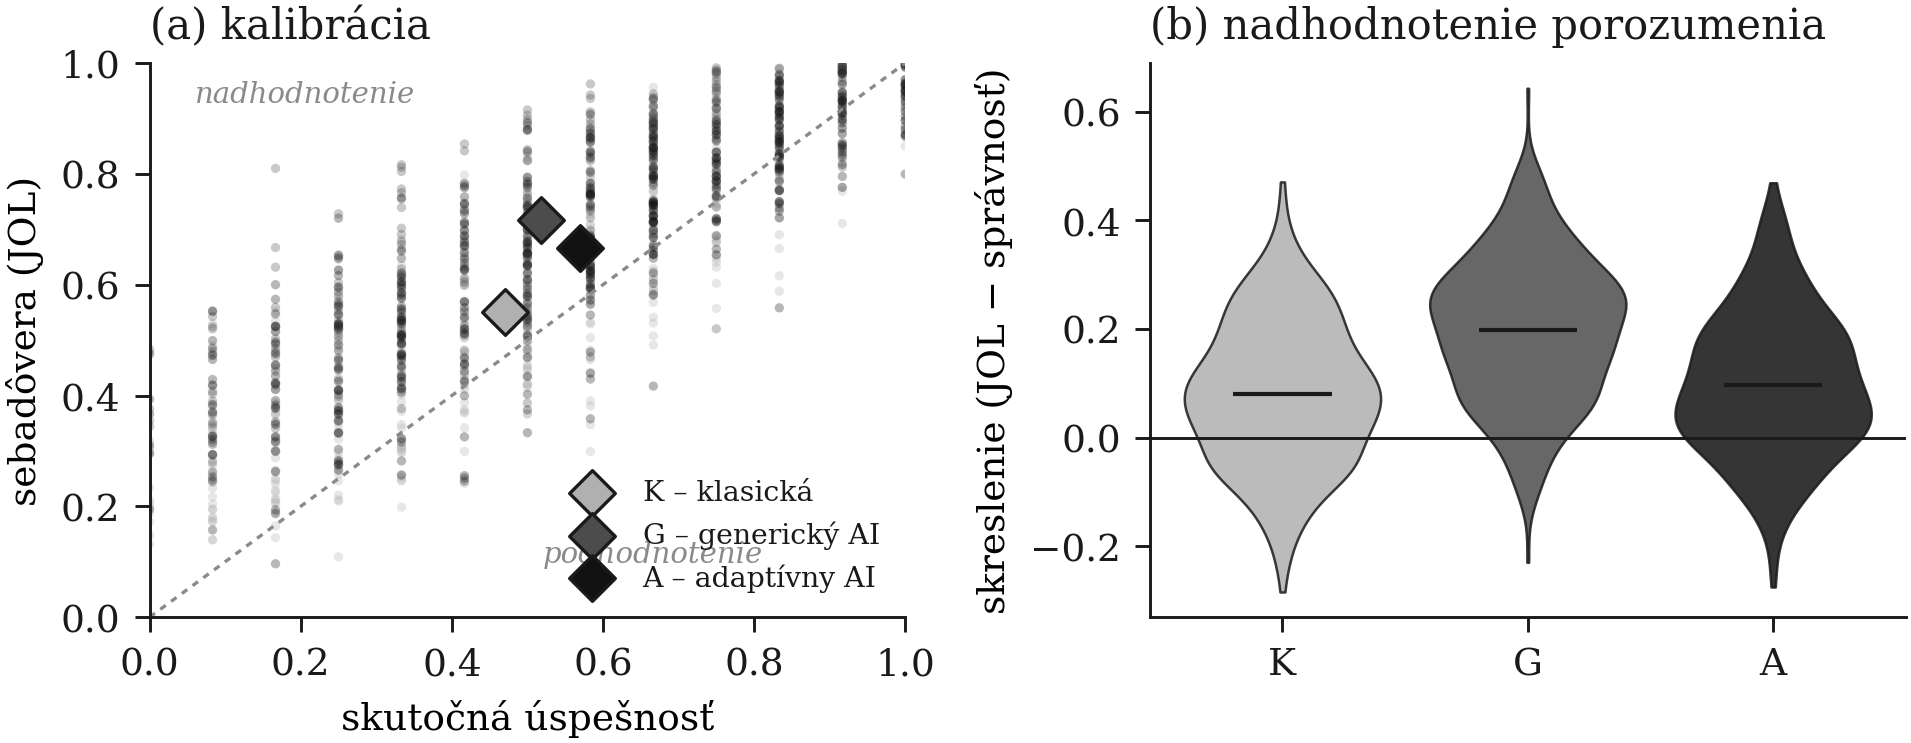
\includegraphics[width=\textwidth]{assets/images/fig_calibration.png}
    \caption{(a)~Kalibrácia: sebadôvera oproti skutočnej úspešnosti; body nad uhlopriečkou znamenajú nadhodnotenie. Kosoštvorce sú priemery podmienok. (b)~Rozdelenie kalibračného skreslenia.}
    \label{fig:kalibracia}
\end{figure}

Kalibračné skreslenie je $\calBiasK$ v podmienke $K$, $\calBiasA$ v podmienke $A$ a $\calBiasG$ v podmienke $G$. Rozdiel $G-K$ je $\calBiasGK$ ($p<0{,}001$) a rozdiel $G-A$ je $\calBiasGA$ ($p<0{,}001$). Žiaci po hodine s generickým nástrojom teda očakávajú, že odpovedali správne približne na trinástinu viac otázok, než v skutočnosti; v absolútnych číslach ide o dve položky zo šestnástich.

Zaujímavý je nález, ktorý simulácia produkuje bez toho, aby bol priamo vložený: \emph{rozlišovacia schopnosť} (Goodman--Kruskalova $\gamma$) sa medzi podmienkami prakticky nelíši ($\calGammaK$ v $K$; $\calGammaG$ v $G$; $\calGammaA$ v $A$) a žiadny z kontrastov nie je významný. Žiaci v podmienke $G$ teda nestratili schopnosť rozoznať, ktorým vlastným odpovediam veriť; posunula sa len ich úroveň sebadôvery ako celok. Toto rozlíšenie je prakticky dôležité, pretože naznačuje, že nápravou nie je učiť žiakov lepšie rozlišovať, ale posunúť ich celkovú kalibráciu~--- napríklad tým, že dostanú spätnú väzbu o rozdiele medzi očakávaným a skutočným výsledkom. Ide o lacnú intervenciu s jasným cieľom.

Formálny test disociácie~--- interakcia podmienky s typom ukazovateľa na štandardizovaných hodnotách~--- vychádza $\disG$ ($p<0{,}001$) pre $G$ oproti $K$ a $\disA$ ($p<0{,}001$) pre $A$ oproti $K$. Obe podmienky s nástrojom teda vykazujú väčší rozstup medzi pocitom a výkonom než klasická výučba, najväčší však generický nástroj.

\section{Mechanizmus: čo z neho randomizácia unesie}
\label{sec:vysledky-mechanizmus}

Automatický klasifikátor promptov dosiahol na kotviacom súbore v päťnásobnej krížovej validácii $\kappa=\peqiCvKappa$; samotné rozhodovacie pravidlo bez učenia dosiahlo $\kappa=\peqiRuleKappa$. Simulované dvojité kódovanie dvoma hodnotiteľmi dáva Krippendorffovu $\alpha=\peqiAlpha$, čo prekračuje stanovenú hranicu $0{,}80$. Podstatné je, že $\peqiAdjacent\,\%$ chýb klasifikátora je posunom o jedinú susednú úroveň; pri ordinálnej škále to vedie k útlmu účinku, nie k jeho prevráteniu.

Hodnoty indexu sa medzi podmienkami rozchádzajú výrazne: $\mathrm{PEQI}=\procPeqiG$ v podmienke $G$ oproti $\procPeqiA$ v podmienke $A$; miera offloadingu $\procOfflG$ oproti $\procOfflA$; miera doslovného prevzatia výstupu $\procVtrG$ oproti $\procVtrA$; medián času do prvého promptu $\procTfirstG$~sekúnd oproti $\procTfirstA$~sekundám a $\procNprG$ oproti $\procNprA$ promptov na žiaka a hodinu.

Mediačný model (obrázok~\ref{fig:peqi}~c) dáva dráhu $a=\medA$ ($p<0{,}001$), dráhu $b=\medB$ ($\mathrm{SE}=\medBse$; $p=\medBp$), priamy účinok $c'=\medDirect$ a nepriamy účinok $\medIndirect$ s $95\,\%$ intervalom $[\medIndLo;\ \medIndHi]$. Celkový účinok je $\medTotal$, rozklad \emph{celkový $=$ priamy $+$ nepriamy} platí presne a podiel mediácie je $\medProp$. Ak sa dráha $b$ odhaduje očistená o okamžité učenie, vychádza $\medBnet$ ($p=\medBnetP$): kvalita promptov predpovedá to, čo \emph{prežije}, nad rámec toho, čo žiak vedel na konci hodiny.

To všetko však stojí na predpoklade, ktorý dizajn nedodáva (časť~\ref{sec:identifikacia}). Preto trojica odhadov v tabuľke~\ref{tab:triangulacia}.

\begin{table}[H]
\centering
\caption{Tri odhady tej istej dráhy pod tromi rôznymi predpokladmi}
\label{tab:triangulacia}
\small
\begin{tabularx}{\textwidth}{@{}l c c X@{}}
\toprule
\textbf{Postup} & \textbf{Odhad} & \textbf{95\,\% IS} & \textbf{Predpoklad, ktorý musí platiť} \\
\midrule
Mediačný model & $\medB$ & $[\medBlo;\ \medBhi]$ & žiadna nepozorovaná spoločná príčina PEQI a vybavenia \\
Inštrumentálna premenná & $\ivEst$ & $[\ivLo;\ \ivHi]$ & podmienka pôsobí na vybavenie \emph{len} cez PEQI \\
Dávková závislosť v $G$ & $\doseEst$ & $[\doseLo;\ \doseHi]$ & (nič neidentifikuje; len linearita) \\
\bottomrule
\end{tabularx}
\end{table}

Tri odhady sa pohybujú v rozpätí $\triSpread$ a všetky sú kladné; naprieč \valReps{} simulovanými štúdiami je medián rozpätia $\valSpreadMed$ a deväťdesiaty percentil $\valSpreadPninety$. $F$-štatistika prvého stupňa je $\ivF$, takže inštrument nie je slabý; jeho sila je v tomto dizajne daná tým, že pedagogická vrstva posúva kvalitu promptov o takmer jeden a pol smerodajnej odchýlky. Zhoda troch odhadov opierajúcich sa o tri \emph{rôzne} predpoklady je podstatne silnejším dôkazom než ktorýkoľvek z nich samostatne, pretože každý z predpokladov by musel byť porušený tak, aby výsledok posunul rovnakým smerom a približne rovnako.

\paragraph{Ktorý z troch odhadov je najpresnejší a prečo je to prekvapivé.} V tomto výbere je interval mediačného odhadu zreteľne najširší a jeho $p$-hodnota nedosahuje hladinu významnosti, kým odhad inštrumentálnou premennou je tesný. Nejde o zvláštnosť výberu: naprieč \valReps{} štúdiami má mediačný odhad smerodajnú odchýlku $\valBmedSd$ a inštrumentálny $\valBivSd$, teda zhruba polovičnú. To je opak toho, čo sa od inštrumentálnych premenných zvyčajne čaká~--- bývajú neefektívne, lebo prvý stupeň býva slabý. Tu je prvý stupeň mimoriadne silný, pretože manipulácia posúva mediátor takmer o jeden a pol smerodajnej odchýlky, a slabý inštrument sa nevyskytol ani raz.

Z toho vyplýva praktické odporúčanie pre podobné dizajny: ak už experiment obsahuje randomizovanú manipuláciu, ktorá pôsobí prevažne na jednu procesnú premennú, je výhodnejšie použiť ju ako inštrument než sa spoliehať na mediačný model. Odhad je presnejší a jeho identifikačný predpoklad je aspoň sčasti pod kontrolou dizajnu, kým predpoklad mediačného modelu nie je pod kontrolou vôbec.

\paragraph{Ako krehké to je.} Analýza citlivosti (obrázok~\ref{fig:dag}~b) dáva $\rho^\ast = \rhoStar$. Nepozorované zmätenie, ktoré by vysvetľovalo približne \rhoPct{}~\% zvyškového rozptylu \emph{aj} kvality promptov \emph{aj} odloženého vybavenia, by nepriamy účinok zredukovalo na nulu. Podľa vopred stanoveného pravidla z časti~\ref{subsec:citlivost} ($\rho^\ast < 0{,}15$) je mediačné zistenie \textbf{krehké}. Nejde o zvláštnosť tohto výberu: naprieč \valReps{} simulovanými štúdiami je priemerné $\rho^\ast$ rovné $\valRhoMean$ a pod prahom $0{,}15$ padne v \valRhoFragile\,\% prípadov. Pri účinku tejto veľkosti teda mediačná cesta \emph{sústavne} nedosahuje úroveň dôkazu, ktorú by sme od záveru práce žiadali~--- a to je vlastnosť problému, nie chyba analýzy.

To je nepríjemný, ale správny záver, a má dva dôsledky. Po prvé, mediačné tvrdenie nepatrí medzi závery práce a v tejto podobe tam ani nebude uvedené. Po druhé, práve preto má odhad inštrumentálnou premennou samostatnú hodnotu: nestojí na sekvenčnej ignorovateľnosti a citlivosť na $\rho$ sa naň nevzťahuje. Cenou je, že stojí na podmienke vylúčenia, ktorú dizajn robí hodnovernou, no nie istou~--- adaptívne poradie úloh je kanál, ktorý cez kvalitu promptov nevedie. Odhad $\ivEst$ preto vykazujeme ako \emph{hornú hranicu} veľkosti dráhy $b$.

Zostáva to, čo randomizácia unesie bez výhrad: hypotéza H6a, teda rozdiel $A-G$ na odloženom teste $\conDelAG$ ($p<0{,}001$). Adaptívna vrstva zlepšuje trvalé osvojenie oproti generickému nástroju. \emph{Že} sa tak deje, je preukázané dizajnom; \emph{ako} sa tak deje, je podložené triangulovane a s vyčíslenou krehkosťou.

\section{Chyba merania mediátora: čo by spôsobila a ako sa ošetruje}
\label{sec:vysledky-merania}

Predchádzajúca časť zaobchádzala s PEQI ako s pozorovanou veličinou. Nie je ňou. Táto časť spúšťa model chyby z časti~\ref{sec:diferencialna} na dátach so \emph{známou} chybou a overuje, že tvrdenia T1--T3 platia aj v kóde, nielen na papieri.

\subsection{Overenie troch tvrdení}

Do generujúceho modelu vkladáme $a=\measApath$, $b=\measBpath$, diferenciálnu chybu $\delta=\measDelta$ a klasickú chybu so spoľahlivosťou $\lambda=\measLambda$, pri platnej vylučovacej podmienke. Skutočný nepriamy účinok je teda $ab=\measItt$. Tabuľka~\ref{tab:mererr} porovnáva, čo z neho jednotlivé odhady vrátia.

\begin{table}[H]
\centering
\caption{Čo diferenciálna a klasická chyba mediátora urobia s každým odhadom ($n=400\,000$)}
\label{tab:mererr}
\small
\begin{tabularx}{\textwidth}{@{}l c c X@{}}
\toprule
\textbf{Veličina} & \textbf{Skutočná} & \textbf{Odhadnutá} & \textbf{Prečo} \\
\midrule
Redukovaná forma $ab$ & \measItt & \measItt & neobsahuje mediátor vôbec \\
Dráha $b$ (IV) & \measBpath & \measIvObs & útlm faktorom $a/(a+\delta)=\measIvAtten$ \\
Nepriamy účinok (mediácia) & \measItt & \measMedObs & nafúknutie $\times\measMedInflate$, útlm $\times\measLambda$ \\
\bottomrule
\end{tabularx}
\end{table}

Prvý riadok je najdôležitejší a zároveň najmenej samozrejmý. Redukovaná forma je \emph{numericky totožná} s hodnotou, ktorá by vyšla pri dokonale meranom mediátore~--- nie približne, ale na všetky desatinné miesta, pretože mediátor do nej nevstupuje. Z toho plynie vykazovacie pravidlo z časti~\ref{sec:diferencialna}: mechanizmové výsledky sa uvádzajú vedené redukovanou formou a až za ňou účinkom na jednotku PEQI.

Druhý riadok obracia bežnú intuíciu. Diferenciálna chyba nafúkne prvý stupeň~--- pedagogická vrstva sa javí, že hýbe kvalitou promptov \emph{viac}, než hýbe~--- a tým odhad účinku na jednotku \emph{zmenší}. Výskumník, ktorý by väčší prvý stupeň čítal ako dobrú správu, by čítal príznak artefaktu ako dôkaz sily manipulácie.

\paragraph{Prípad, ktorý žiadna diagnostika nevidí.} Tretí riadok obsahuje dve skreslenia opačného smeru, takže existuje hodnota $\delta$, pri ktorej sa presne zrušia. Pri tu použitých parametroch je to $\delta=\measCancel$. Vtedy je mediačný odhad nezaujatý, hoci dráha $a$ aj dráha $b$ sú nesprávne. Simulácia to potvrdzuje a je to dôvod, prečo sa audit nedá nahradiť kontrolou výstupov: bodový odhad v tomto prípade vyzerá bezchybne.

\subsection{Diagnostický podiel}

Rovnica~\eqref{eq:ratio} predpovedá pomer mediačného a inštrumentálneho odhadu $(1+\delta/a)\lambda = \measRatioPred$. Simulácia dáva tú istú hodnotu v rámci simulačnej chyby. Keď sa do tých istých dát pridá zmätenie mediátora s výsledkom na úrovni $\rho=0{,}35$, pomer vyskočí na $\measRatioConf$.

To je použiteľná diagnostika, nie iba algebraická poznámka. Rozdiel medzi oboma odhadmi \emph{do výšky} $(1+\hat\delta/\hat a)\hat\lambda$ je vysvetlený chybou merania a nevyžaduje si iný výklad. Rozdiel \emph{nad} túto hodnotu chybou merania vysvetliť nemožno a ukazuje na zmätenie, ktoré ohraničuje $\rho^\ast$. Triangulácia z tabuľky~\ref{tab:triangulacia} tým získava kvantitatívne očakávanie: doteraz sa o zhode troch odhadov dalo povedať len to, že je väčšia alebo menšia.

\subsection{Korekcia obnoví vložené hodnoty}

Na tých istých dátach s vloženým $\delta=\measDelta$ dáva neopravený odhad dráhu $a=\corrNaiveA$ namiesto $\corrTrueA$ a dráhu $b=\corrNaiveB$ namiesto $\corrTrueB$. Dvojkroková korekcia~--- odčítanie $\hat\delta A$ od mediátora, potom regresná kalibrácia koeficientom $1/\hat\lambda$~--- vracia $a=\corrCalA$ a $b=\corrCalB$, teda obe vložené hodnoty v rámci $0{,}02$.

Stojí za zaznamenanie, ktorá časť opravy urobí akú prácu. Prvý krok opravuje dráhu $a$ a nechá $b$ nedotknuté, pretože $\delta$ je kolineárne s podmienkou a z koeficientu pri mediátore sa vykráti. Druhý krok opravuje $b$ a nechá $a$ nedotknuté. Vykonať druhý bez prvého by znamenalo deliť správny koeficient spoľahlivosťou~--- teda pokaziť to, čo bolo v poriadku, a nechať pokazené tak.

\subsection{Rozsah auditu}

Audit s \audN{} promptmi na podmienku má pri $\kappa$ na úrovni prijímacieho prahu plánu silu $\audPower$ na detekciu $\delta=\audDelta$ a odhaduje ho nezaujato so smerodajnou chybou $\audSe$. Úplná krivka sily je v tabuľke~\ref{tab:audit}. Náklad je približne tri hodiny práce dvoch kódovateľov, čo je vo vzťahu k tomu, čo audit chráni, zanedbateľné.

\paragraph{Čo by sa stalo bez neho.} Ak by sa audit nespravil a zostatková diferenciálna chyba by bola veľkosti $\venDeltaBefore$, teda tej, ktorú mala pôvodná verzia klasifikátora, bol by prvý stupeň nafúknutý natoľko, že by inštrumentálny odhad klesol pod polovicu skutočnej hodnoty~--- a práca by uzavrela, že na kvalite promptov záleží podstatne menej, než v skutočnosti záleží. Tento konkrétny scenár je už uzavretý (časť~\ref{sec:dominancia}); audit je tu preto, že uzavretý je len na kotviacom súbore, a kotviaci súbor nie je trieda.


\section{Procesné ukazovatele}

Procesné ukazovatele sú v pláne uvedené ako sekundárne výsledky, takže sa odhadujú a korigujú ako ktorýkoľvek iný sekundárny výsledok. Deklarovať ukazovateľ a nikdy ho nevykázať je tichá verzia selektívneho vykazovania.

\begin{table}[H]
\centering
\caption{Procesné ukazovatele, kontrast $A$ oproti $G$ (korekcia miery falošných objavov)}
\label{tab:proces}
\small
\begin{tabular}{@{}lrrrrr@{}}
\toprule
\textbf{Ukazovateľ} & \textbf{$G$} & \textbf{$A$} & \textbf{Rozdiel} & \textbf{$d$} & \textbf{$q$} \\
\midrule
PEQI & \procPeqiG & \procPeqiA & $\procPeqiDiff$ & $\procPeqiD$ & $<0{,}001$ \\
miera offloadingu & \procOfflG & \procOfflA & $\procOfflDiff$ & $\procOfflD$ & $<0{,}001$ \\
doslovné prevzatie výstupu (VTR) & \procVtrG & \procVtrA & $\procVtrDiff$ & $\procVtrD$ & $<0{,}001$ \\
vlastný pokus pred pomocou (ABHR) & \procAbhrG & \procAbhrA & $\procAbhrDiff$ & $\procAbhrD$ & $<0{,}001$ \\
čas do prvého promptu ($T_1$, s) & \procTfirstG & \procTfirstA & $\procTfirstDiff$ & $\procTfirstD$ & $<0{,}001$ \\
počet promptov na hodinu & \procNprG & \procNprA & $\procNprDiff$ & $\procNprD$ & $<0{,}001$ \\
\bottomrule
\end{tabular}
\end{table}

\paragraph{Ako tieto čísla čítať a ako ich nečítať.} Veľkosti účinkov sú tu rádovo väčšie než pri učebných výsledkoch a bolo by chybou vydávať to za silu zistenia. Tieto ukazovatele sú z veľkej časti \emph{kontrolami manipulácie}, nie objavmi: adaptívna vrstva zo svojej definície nevydá hotové riešenie, takže je v nej takmer čo prevziať, a bránu vlastného vysvetlenia nemožno obísť, takže vlastný pokus pred pomocou je vynútený. Ak by tieto rozdiely nevyšli, znamenalo by to, že manipulácia nefungovala, a zvyšok analýzy by nemal zmysel.

Informačná hodnota je preto inde: v tom, že \emph{tieto veľké procesné rozdiely sa neprekladajú do rovnako veľkých rozdielov v učení}. Adaptívna vrstva zmení spôsob práce o dve až štyri smerodajné odchýlky, a rozdiel v trvalom osvojení je $d=\conDelAGD$. Zmeniť správanie žiaka je teda ľahšie než zmeniť to, čo si odnesie~--- čo je striedmejší záver, než k akému by procesné čísla samy zvádzali.

Praktický význam má ABHR. Zo všetkých ukazovateľov je najzrozumiteľnejší učiteľovi, nevyžaduje klasifikáciu textu a dá sa merať aj bez zachytávania promptov~--- postačujú časové značky cvičného rozhrania. Ak by sa index PEQI ukázal ako neprenosný do inej domény, ABHR je najsľubnejší kandidát na náhradu.

\section{Komu generický nástroj škodí najviac}

\begin{figure}[H]
    \centering
    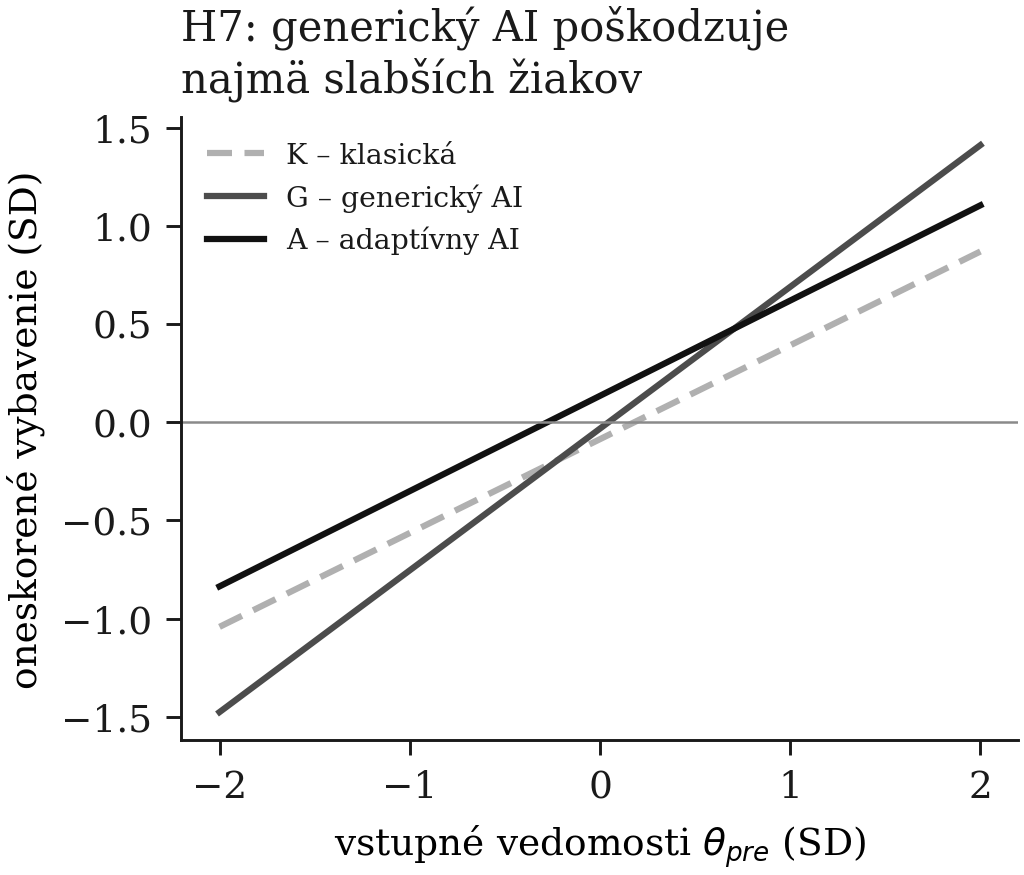
\includegraphics[width=0.62\textwidth]{assets/images/fig_moderation.png}
    \caption{Interakcia podmienky so vstupnými vedomosťami na odloženom teste.}
    \label{fig:moderacia}
\end{figure}

Interakcia podmienky $G$ so vstupnými vedomosťami je $\modG$ ($\mathrm{SE}=\modGse$; $p<0{,}001$); pre podmienku $A$ je nevýznamná. Preložené do jednoduchých sklonov: u žiakov so vstupnými vedomosťami pod priemerom je rozdiel $G-K$ na odloženom teste $\slopeLow$, kým u žiakov nad priemerom je $\slopeHigh$.

Ide o najzávažnejší nález celého obrazca. Generický nástroj nie je rovnomerne mierne škodlivý~--- je výrazne škodlivý pre slabších žiakov a mierne prospešný pre silnejších. Je to presne vzorec, ktorý predpovedá efekt obrátenia expertízy~\cite{kalyuga2003expertise}: žiak s dostatočnými vlastnými schémami dokáže výstup modelu posúdiť a integrovať, žiak bez nich ho môže iba prevziať. Praktický dôsledok je nepríjemný: nástroj poškodzuje práve tých, ktorým má podľa argumentácie o demokratizácii vzdelávania pomáhať najviac. Adaptívna vrstva tento rozdiel vyrovnáva, čo je z hľadiska vzdelávacej politiky najsilnejší argument v prospech jej povinnosti.

\section{Kognitívna záťaž}

Vonkajšia záťaž je v oboch podmienkach s nástrojom nižšia než v klasickej výučbe ($G-K=\loadExtraneousGK$; $A-K=\loadExtraneousAK$ bodu desaťbodovej škály), čo je očakávané~--- nástroj skracuje hľadanie informácie. Germánna záťaž, teda tá časť úsilia, ktorá buduje schémy, je však v podmienke $G$ \emph{nižšia} než v klasickej výučbe ($\loadGermaneGK$) a v podmienke $A$ vyššia ($\loadGermaneAK$); rozdiel $A-G$ je $\loadGermaneAG$ bodu. Vnútorná záťaž sa medzi podmienkami nelíši, čo potvrdzuje, že učivo bolo vo všetkých podmienkach rovnako náročné.

Tento obrazec poskytuje teoretické vysvetlenie hlavného nálezu v jazyku teórie kognitívnej záťaže~\cite{sweller2019twenty}: generický nástroj odstraňuje záťaž nerozlišujúco, vrátane tej produktívnej. Adaptívna vrstva odstraňuje vonkajšiu záťaž, ale germánnu zachováva alebo zvyšuje~--- čo je presne definícia žiaducej ťažkosti~\cite{bjork2011desirable}.

\section{Negatívne kontroly: čo by nás vyviedlo z omylu}
\label{sec:vysledky-negkontroly}

Negatívna kontrola je užitočná len vtedy, keď dokáže zlyhať, a zároveň nezlyháva, keď je všetko v poriadku. Obe vlastnosti sú overené simuláciou na tom istom generujúcom modeli, do ktorého sa zámerne vkladá únik mimo učenia zvolenej veľkosti (tabuľka~\ref{tab:negkontrola}).

Pri nulovom úniku kontrola vyhlási ekvivalenciu v $\falEquivZero$ prípadov a falošne sa ozve v $\falDetectZero$, teda na nominálnej hladine. Pri úniku $0{,}30$~--- čo je veľkosť primárneho účinku $A-K$~--- sa ozve v $\falDetectThirty$ prípadov a ekvivalenciu vyhlási len v $\falEquivThirty$. Kontrola teda robí obe veci, ktoré má robiť, a robí ich v správnych situáciách.

Kontrola nemennou črtou prejde v $\falTraitPass$ prípadov \emph{aj vtedy}, keď je okamžitý kanál naplno otvorený. To nie je slabosť, ale presne zamýšľané rozdelenie práce: matice sa píšu o tri týždne, takže motivácia v deň testu na ne nedosiahne, a ich úlohou je zachytiť poruchu v mašinérii, nie v nálade.

\paragraph{Čo sa tým dá a čo nedá povedať.} Pri 18~triedach je polovičná šírka intervalu na kontrole $\falHalfwidth$. Tvrdenie, ktoré z toho plynie, treba formulovať presne: vylučuje sa kanál mimo učenia dosť veľký na to, aby vysvetlil \emph{celý} primárny účinok. Kanál, ktorý by vysvetlil jeho tretinu, sa nevylučuje~--- pri úniku $0{,}10$ sa kontrola ozve len v $\falDetectTen$ prípadov. Práca to uvádza takto a nie inak, pretože negatívna kontrola, ktorej hranica sa nevykáže, funguje ako ubezpečenie namiesto dôkazu.

\paragraph{Nesamozrejmý praktický dôsledok.} Predĺženie placebo testu pomáha oveľa menej, než by sa čakalo. Polovičná šírka je pri \falShortItems{} položkách $\falHalfShort$, pri \falPlacebo{} $\falHalfwidth$ a pri \falLongItems{} $\falHalfLong$. Príčinou je, že kontrast je vnútroindividuálny, takže zvyškovým rozptylom je zložka žiak\,$\times$\,príležitosť a vzorkovanie položiek je len jednou jej časťou. Pridávať položky teda zmenšuje jednu časť z viacerých. Odporúčanie pre prax je konkrétne: deväť placebo položiek stačí a ďalších sedem je premrhaný čas hodiny.


\section{Kontrola predpokladov a robustnosť}

\paragraph{Prenos medzi periódami.} Spoločný test parametrov prenosu nevychádza významne ($\chi^2=\carryStat$; $p=\carryP$), teda vyvážený latinský štvorec s týždenným odstupom funguje tak, ako sa predpokladalo.

\paragraph{Rozklad rozptylu.} Na simulovaných dátach vychádza rozptyl triedy $\varClass$, rozptyl žiaka $\varStudent$ a reziduálny rozptyl $\varResidual$, čo dáva vnútrotriednu koreláciu $\varIcc$ a opakovateľnosť $\varRepeat$. Vnútrotriedna korelácia je nižšia než vložená hodnota $0{,}12$, pretože sa meria na odhadnutej, a teda chybou zaťaženej škále~--- ďalší prejav útlmu.

\paragraph{Analýza len na prvej perióde.} Táto analýza je imúnna voči prenosu, ale používa tretinu dát a má medziskupinový charakter. Kontrast $A-G$ zostáva významný ($d=\robPoneAG$; $p<0{,}001$), rovnako $A-K$ ($d=\robPoneAK$; $p=\robPoneAKP$), zatiaľ čo $G-K$ nie ($d=\robPoneGK$; $p=\robPoneGKP$). Nevýznamnosť posledného je dôsledkom nedostatočnej sily, nie protirečenia: medziskupinový odhad na tretine dát má pre účinok tejto veľkosti silu hlboko pod $0{,}50$. V skutočnej práci to bude nutné uviesť presne takto, aby sa nevýznamnosť nezamieňala s neprítomnosťou účinku~--- a je to zároveň dôvod, prečo je táto analýza len robustnostná a nie primárna.

\paragraph{Ostatné štyri robustnostné analýzy.} Po vylúčení hodín s vernosťou pod 90\,\% (vylúčených \robFidExcl{}~pozorovaní) je kontrast $A-K$ $\robFidAK$ oproti $\conDelAK$ na celej vzorke. Účinok je teda po vylúčení \emph{väčší}, čo je v súlade s tým, že nízka vernosť účinok riedi, a nie s tým, že ho vytvára~--- opačný smer by bol vážnym varovaním. Analýza podľa skutočného priebehu (vylúčených \robPpExcl{}~žiakov, u ktorých sa počas kontrolnej podmienky zachytila komunikácia s asistentom; miera kontaminácie $\robContamRate$\,\%) dáva $A-K = \robPpAK$, teda kontaminácia v tomto rozsahu závery nemení. Na hrubej úspešnosti namiesto Raschovej miery zostáva poradie podmienok zachované, takže záver nezávisí od psychometrického modelu.

Najzaujímavejší je model s náhodným sklonom podmienky podľa triedy. Odhadnutý rozptyl účinku podmienky $A$ medzi triedami je $\robTauCt$, čo po prevode na podiel celkového rozptylu zodpovedá rádovo $\tau^2_{ct} \approx 0{,}03$~--- presne tej hodnote, pri ktorej bola plánovaná veľkosť vzorky. Plánovací predpoklad je tým overený z dát, a nie iba prevzatý z literatúry. Pri skutočnom zbere bude táto hodnota k dispozícii po prvej perióde a umožní prípadnú úpravu plánu ešte pred jeho dokončením.

\section{Chýbajúce údaje a hranica toho, čo dáta unesú}

Výpadok do odloženého testu je $\missRate$\,\%. Nie je náhodný: žiaci, ktorí chýbajú, majú vstupné vedomosti $\missPreMiss$ oproti $\missPreKeep$ u ostatných ($t=\missT$; $p<0{,}001$). Predpoklad úplnej náhodnosti (MCAR) je teda zamietnutý, čo je presne dôvod, prečo sú vstupné vedomosti v modeli a nielen vykázané v tabuľke: zmiešaný model je nezaujatý za slabšieho predpokladu MAR, podmienene na modelovaných premenných.

Viacnásobná imputácia (20~imputácií) dáva $A-K = \missMiAK$ a $G-K = \missMiGK$, teda prakticky totožné s analýzou kompletných prípadov. To hovorí, že pri platnosti MAR výpadok závery nemení.

\paragraph{Nepriaznivý scenár a jeho výsledok.} Úmyselne nepriaznivý scenár~--- chýbajúcim hodnotám v podmienke $A$ sa priradí najhorší a v podmienkach $K$ a $G$ najlepší pozorovaný kvartil~--- znižuje $A-K$ z $\conDelAK$ na $\missWorstAK$. Kontrast $G-K$ zostáva $\missWorstGK$.

Pri výpadku okolo desatiny teda hlavné tvrdenie prežije aj nepriaznivý scenár, hoci s viditeľne menším účinkom. To je dobrá správa s jednou podmienkou: platí len pokým je výpadok malý. Nepriaznivý scenár je totiž v podstate lineárny v miere výpadku, takže pri dvojnásobnom úbytku by účinok klesol na hranicu praktickej významnosti.

Praktický dôsledok je konkrétny a nie je štatistický: udržanie účasti na odloženom teste je pre túto štúdiu dôležitejšie než získanie ďalších dvoch tried. Preto je v pláne zberu odložený test viazaný na bežnú vyučovaciu hodinu, a nie na dobrovoľný termín, a preto sa miera výpadku sleduje priebežne ako ukazovateľ kvality zberu, nie až pri analýze.

\section{Operačné charakteristiky celého plánu}
\label{sec:operacne}

Doteraz uvedené čísla pochádzajú z \emph{jedného} výberu z generujúceho modelu. To stačí na overenie, že plán beží a že obnoví vložené parametre, ale nestačí na žiadnu vetu o tom, ako veci dopadli. Bodový odhad kontrastu, ktorého skutočná hodnota je blízka nule, padne pri jednom výbere raz na jednu a raz na druhú stranu nuly. Písať prózu okolo znamienka takého odhadu znamená písať o náhode.

Rozhodovacie tvrdenia sa preto opierajú o rozdelenie naprieč \valReps{} simulovanými štúdiami, a jeden výber slúži už len na ukážku toho, ako výstup vyzerá.

\subsection{Ako často plán dospeje k správnemu rozhodnutiu}

\begin{table}[H]
\centering
\caption{Podiel z \valReps{} simulovaných štúdií, v ktorých plán dospel k danému záveru ($J=18$)}
\label{tab:operacne}
\small
\begin{tabularx}{\textwidth}{@{}l c X@{}}
\toprule
\textbf{Rozhodnutie} & \textbf{Podiel} & \textbf{Poznámka} \\
\midrule
$A>K$ na odloženom teste (H3a) & \valAK & vložený účinok $d=\valDakTrue$ \\
$A>G$ na odloženom teste (H6a) & \valAG & najsilnejší z troch kontrastov \\
$G\equiv K$ (TOST, H3b) & \valEq & viazané obmedzenie celej rodiny \\
\midrule
\textbf{všetky tri súčasne} & \textbf{\valAll} & výsledok, o ktorom práca argumentuje \\
\bottomrule
\end{tabularx}
\end{table}

Hodnota \valAll{} pre celú rodinu je nezávislým potvrdením analýzy sily z časti~\ref{sec:sila}, ktorá pre rovnaké usporiadanie dáva \powFameighteen. Dve simulácie napísané oddelene, s odlišnou implementáciou aj odlišnými predpokladmi o tom, čo treba modelovať, sa zhodujú na dve stotiny. To je silnejší dôkaz správnosti výpočtu než ktorákoľvek z nich sama.

\subsection{Nestrannosť a pokrytie intervalov}

\begin{table}[H]
\centering
\caption{Vychýlenie odhadov a pokrytie 95\,\% intervalov naprieč \valReps{} štúdiami}
\label{tab:nestrannost}
\small
\begin{tabular}{@{}lccccc@{}}
\toprule
\textbf{Kontrast} & \textbf{Vložené $d$} & \textbf{Priemer} & \textbf{SD} & \textbf{Vychýlenie} & \textbf{Pokrytie} \\
\midrule
$A-K$ & \valDakTrue & \valDakMean & \valDakSd & \valDakBias & \valCovAK \\
$G-K$ & \valDgkTrue & \valDgkMean & \valDgkSd & \valDgkBias & \valCovGK \\
$A-G$ & \valDagTrue & \valDagMean & \valDagSd & \valDagBias & --- \\
\bottomrule
\end{tabular}
\end{table}

Vychýlenie je vo všetkých troch prípadoch pod dve stotiny, teda plán je prakticky nestranný. Pokrytie intervalov je naopak \emph{vyššie} než nominálnych $0{,}95$. Interval je teda širší, než by musel byť, čo je pri malom počte zhlukov žiaduce a zodpovedá tomu, čo sme už videli na chybe prvého druhu: klastrovo robustný test s $J-1$ stupňami voľnosti je konzervatívny. Cenou za túto opatrnosť je mierne nižšia sila, ktorá je v analýze sily už započítaná.

\subsection{Nestabilita znamienka}

Kontrast $G-K$ má vloženú hodnotu $d=\valDgkTrue$, teda takmer nulovú. Naprieč \valReps{} štúdiami vyjde jeho bodový odhad \emph{kladný} v \valSignFlip\,\% prípadov. Z toho vyplýva pravidlo, ktoré v práci dodržiavame: o znamienku tohto kontrastu sa netvrdí nič. Tvrdenie, ktoré dáta unesú, je tvrdenie o ekvivalencii, a to je formulované testom voči vopred stanovenej hranici, nie pohľadom na to, ktorým smerom odhad práve ukazuje.

Ide o drobnosť s veľkými dôsledkami. Prvá verzia tejto kapitoly obsahovala vetu o tom, že generický nástroj „klesol pod úroveň klasickej výučby“. Bola pravdivá pre vtedajší výber a nepravdivá pre nasledujúci; zmena, ktorá ju obrátila, bolo pridanie jednej premennej do generujúceho modelu. Veta bola odstránená, nie prepísaná.

\subsection{Mechanizmus naprieč štúdiami}

Odhad dráhy $b$ mediačným modelom má priemer \valBmed{} so smerodajnou odchýlkou \valBmedSd, odhad inštrumentálnou premennou priemer \valBiv{} so smerodajnou odchýlkou \valBivSd. Za povšimnutie stojí, že \emph{inštrumentálny odhad je presnejší}, hoci sa zvyčajne očakáva opak: inštrumentálne premenné bývajú neefektívne, keď je prvý stupeň slabý. Tu je prvý stupeň mimoriadne silný, pretože pedagogická vrstva posúva kvalitu promptov o takmer jeden a pol smerodajnej odchýlky, a slabý inštrument sa nevyskytol ani v jednej zo \valReps{} štúdií.

Interval pre nepriamy účinok vylučuje nulu v \valIndirect{} prípadov. Prah citlivosti $\rho^\ast$ má priemer \valRhoMean{} a pod hranicou $0{,}15$ padne v \valRhoFragile\,\% štúdií.

Posledné číslo je najdôležitejšie v celej kapitole. Znamená, že pri účinku veľkosti, akú literatúra naznačuje, mediačná cesta \emph{sústavne} nedosiahne úroveň dôkazu, ktorú by sme od záveru práce žiadali. Nejde o nedostatok tejto vzorky ani o chybu analýzy~--- je to vlastnosť problému. Mediačný odhad je zo svojej podstaty citlivý na nepozorované zmätenie a pri stredne veľkých účinkoch stačí na jeho zvrátenie zmätenie, ktoré je v školskej triede hodnoverné. Preto má odhad inštrumentálnou premennou samostatnú hodnotu a preto mechanizmové tvrdenie nepatrí do konfirmačnej rodiny.

\section{Čo simulácia odhalila a čo sa vďaka nej zmenilo}
\label{sec:co-odhalila-simulacia}

\begin{enumerate}[nosep]
    \item \textbf{Singularita v kódovaní prenosu.} Pôvodný zápis modelu obsahoval samostatnú úroveň „bez prenosu“ pre prvú periódu. Tá je dokonale kolineárna s indikátorom prvej periódy, takže model vracal nekonečné štandardné chyby~--- teda by bol pri reálnych dátach nepoužiteľný. Riešením je priradenie referenčnej úrovne prvej perióde~\cite{senn2002crossover}.
    \item \textbf{Nedostatočná dĺžka odloženého testu.} Pri ôsmich položkách na tému vychádzala spoľahlivosť $0{,}63$, čo je pre primárny ukazovateľ neprijateľné. Rozšírenie na dvanásť položiek ju zvýšilo na $0{,}68$ pri zachovaní jednej vyučovacej hodiny na administráciu.
    \item \textbf{Veľkosť vzorky pre tvrdenie o ekvivalencii.} Pôvodný plán počítal s 12~triedami podľa sily testu nadradenosti. Simulácia ukázala, že pri tejto veľkosti test ekvivalencie~--- ktorý je pre prácu dôležitejší~--- zlyháva. Cieľová veľkosť bola zvýšená na 18~tried.
    \item \textbf{Konfirmačná rodina obsahovala hypotézu, ktorú dizajn neidentifikuje.} Pôvodne bola medzi primárne zaradená mediačná hypotéza. Pri písaní identifikačnej časti sa ukázalo, že randomizácia prideľuje podmienku a nie kvalitu promptov, takže mediačné tvrdenie stojí na predpoklade, ktorý dizajn nedodáva, a do konfirmačnej rodiny nepatrí. Rodina bola prepracovaná na tri tvrdenia, ktoré randomizácia identifikuje a ktoré môžu zlyhať, a mechanizmus bol presunutý do triangulovaného režimu s analýzou citlivosti.
    \item \textbf{Ekvivalencia testových foriem nebola v pôvodnom pláne vykonávaná.} Text sľuboval prevod oboch foriem na spoločnú škálu cez kotviace položky, ale kód kalibroval každú formu samostatne. Na simulovaných dátach by rozdiel medzi okamžitým a odloženým skóre bol artefaktom centrovanie. Zavedená bola súbežná kalibrácia, ktorá zabudnutie obnoví s chybou $0{,}044$ logitu a navyše zvýši spoľahlivosť odloženého testu z $0{,}68$ na $0{,}73$.
    \item \textbf{Kritérium presnosti pre mechanizmus chýbalo úplne.} Pôvodne sa plánovala len sila testu. Simulácia ukázala, že odlíšiteľnosť od nuly je pri tomto inštrumente takmer istá už pri deviatich triedach, kým dostatočná presnosť nie~--- pravdepodobnosť dosť úzkeho intervalu je tam $0{,}31$. Kritérium šírky intervalu bolo doplnené do plánu.
    \item \textbf{Klasifikátor mediátora bol zameniteľný formulkou, a to systematicky v prospech jednej podmienky.} Prvá verzia priraďovala najvyššiu úroveň každému promptu s epistemickou formulkou. Keďže adaptívna vrstva takú formulku od žiakov \emph{vyžaduje}, meranie mediátora by bolo skreslené práve tou manipuláciou, ktorú má merať~--- o $\venDeltaBefore$ na prompt, teda viac než dvojnásobok hľadaného medzipodmienkového rozdielu. Chyba bola nájdená pokusom o jej zneužitie, nie čítaním kódu. Pravidlá boli prepracované (časť~\ref{sec:dominancia}) a zostatková chyba sa odhaduje zaslepeným auditom (časť~\ref{sec:audit}).
    \item \textbf{Dve implementácie tej istej taxonómie sa rozišli.} Oprava predchádzajúceho bodu bola vykonaná v analytickej vrstve a v spracovateľskej vrstve, ktorá skóruje skutočnú prevádzku, zostala nevykonaná. Porovnanie oboch na \venN{} kotviacich a zafarbených promptoch odhalilo deväť nezhôd zo šiestich rôznych príčin. Špecifikácia je odvtedy zafixovaná ako dáta, na ktorých sa obe implementácie musia zhodnúť (časť~\ref{sec:dve-implementacie}).
    \item \textbf{Chýbala falzifikačná kontrola.} Dizajn nemal ukazovateľ, na ktorý podmienka \emph{nesmie} pôsobiť, takže očakávanie od účastníka, zvyšná kapacita a nálada boli od učenia nerozoznateľné. Doplnené boli dve negatívne kontroly s vopred stanoveným rozhodovacím pravidlom (časť~\ref{sec:negativne-kontroly}). Pri ich dimenzovaní sa ukázalo, že prísnejšia hranica by bola nedosiahnuteľná: pri hranici $0{,}20$ by kontrola nevyhlásila ekvivalenciu zhruba v polovici prípadov, \emph{keď je pravda presne nula}.
\end{enumerate}

Okrem toho simulácia vyčíslila tri veci, ktoré bude nutné uviesť pri interpretácii skutočných výsledkov: útlm účinkov chybou merania (približne pätina), skutočnosť, že klastrovo robustný test s $J-1$ stupňami voľnosti je mierne konzervatívny (podiel zamietnutí $0{,}040$ oproti nominálnym $0{,}05$), a krehkosť mediačného zistenia voči nepozorovanému zmäteniu ($\rho^\ast = 0{,}10$).

\paragraph{Poznámka o tom, čo tento postup stál a čo priniesol.} Deväť opráv, z ktorých dve sa týkali samotnej formulácie hypotéz, jedna by spôsobila, že primárny ukazovateľ by nemeral to, čo tvrdí, a dve by boli skreslili mediátor v prospech skúmanej podmienky. Žiadna z nich by sa pri obvyklom postupe~--- napísať plán, zozbierať dáta, potom analyzovať~--- neodhalila v čase, keď je náprava možná. Cena bola niekoľko dní práce pred zberom; alternatívna cena by bola celý školský polrok.

Za zmienku stojí, ako sa jednotlivé chyby našli, pretože to nie je jeden postup, ale tri, a žiadny z nich nenahrádza ostatné. Prvé tri chyby odhalilo \emph{spustenie} plánu na dátach so známou odpoveďou: kód vrátil nekonečnú chybu, nízku spoľahlivosť alebo príliš nízku silu. Ďalšie tri odhalilo \emph{písanie} o tom, čo kód robí~--- nezrovnalosť medzi kapitolou o súčasnom stave a štatistickým plánom sa ukázala pri formulovaní vety, ktorá mala obe zosúladiť. Posledné tri odhalil \emph{pokus o zneužitie vlastného nástroja}: útok formulkou, porovnanie dvoch implementácií proti sebe a otázka, ktorý ukazovateľ by musel zostať nehybný, keby zistenie bolo pravdivé. Tretí postup bol najproduktívnejší a v metodických prácach sa vyskytuje najzriedkavejšie.

\section{Ako sa táto kapitola premení na kapitolu s výsledkami}

Po zbere dát sa zmenia presne dve veci. Po prvé, vstupný súbor: namiesto výstupu z generujúceho modelu sa načíta skutočný dátový súbor s totožnou štruktúrou stĺpcov. Po druhé, upozornenie na začiatku kapitoly sa odstráni. Kód analýzy, štruktúra tabuliek, obrázky ani poradie oddielov sa nemenia~--- to je zmyslom uzavretia plánu pred zberom.

Akékoľvek analýzy, ktoré v pláne nie sú, budú v texte výslovne označené ako exploratívne a ich $p$-hodnoty sa nebudú interpretovať konfirmačne. Rovnako bude vykazovaný každý prípad, keď sa skutočný priebeh odchýlil od plánu (napríklad nižší počet získaných tried), spolu s dôsledkom pre silu testu.
